\documentclass{article}
\usepackage{graphicx}
\usepackage{amsmath}
\usepackage{booktabs}
\usepackage{array}
\usepackage{hyperref}
\usepackage{float}
\usepackage{tikz}
\usepackage{circuitikz}
\usepackage{karnaugh-map}
\usepackage{subcaption}
\usepackage{listings}
\usepackage{xcolor}

\title{EE1501 Assignment 2}
\author{Arjun Pavanje}
\date{April 2025}

\begin{document}
\definecolor{codegreen}{rgb}{0,0.6,0}
\definecolor{codegray}{rgb}{0.5,0.5,0.5}
\definecolor{codepurple}{rgb}{0.58,0,0.82}
\definecolor{backcolour}{rgb}{0.95,0.95,0.92}
\lstdefinestyle{style}{
    backgroundcolor=\color{backcolour},   
    commentstyle=\color{codegreen},
    keywordstyle=\color{magenta},
    numberstyle=\tiny\color{codegray},
    stringstyle=\color{codepurple},
    basicstyle=\ttfamily\footnotesize,
    breakatwhitespace=false,         
    breaklines=true,                 
    captionpos=b,                    
    keepspaces=true,                 
    numbersep=5pt,                  
    showspaces=false,                
    showstringspaces=false,
    showtabs=false,                  
    tabsize=2,
    literate={~}{\texttt{\char126}}1,
}
\maketitle
\section{Convolution}
\begin{itemize}
    \item \textbf{Inputs:} Two 8-bit vectors 
    \begin{itemize}
        \item \texttt{[3:0] x [7:0]}
        \item \texttt{[3:0] h [7:0]}.
    \end{itemize}
    \item \textbf{Outputs:} Vector $\texttt{[3:0] y [15:0]}$, which contains the result of $x \ast h$
\end{itemize}

\subsection*{Approach:} 
Convolution of two vectors is basically polynomial multiplication where coeffecients of the polynomials are elements of the vector. Output vector will be given by,
\[
y[n] = \sum_{k=0}^{7} x[k] \cdot h[n-k]
\]
$n$ varies from $0$ to $15$ (vectors are indexed from $0$). All elements of $y$ are also $4-$bit numbers, overflow is ignored.
\subsection*{Code}
\begin{lstlisting}[style=style]
module convolvolution (
  input  [3:0] x [7:0],   
  input  [3:0] h [7:0],   
  output reg [3:0] y [14:0]   
);

integer i, k, j;
always @(*) begin
  for (i = 0; i < 15; i = i + 1) begin 
    y[i] = 4'd0; // initalizing each element to 0
  end
  for (j=0; j < 8; j = j + 1) begin
    for (k = 0; k < 8; k = k + 1) begin
      y[j+k] += x[j]*h[k];
    end
  end
end
endmodule
\end{lstlisting}
\subsection*{Testbench}
\begin{lstlisting}[style=style]
module tb_convolvolution;
reg [3:0] x[7:0];
reg [3:0] h[7:0];
wire [3:0] y[14:0];

convolvolution dut(.x(x), .h(h), .y(y));

initial begin
  $dumpfile("convolvolution.vcd");
  $dumpvars(0, tb_convolvolution);

  for (integer i = 0; i < 8; i++) begin
    $dumpvars(0, tb_convolvolution.x[i]);
    $dumpvars(0, tb_convolvolution.h[i]);
  end

  for (integer i = 0; i < 15; i++) begin
    $dumpvars(0, tb_convolvolution.y[i]);
  end

  $monitor("x = [%d, %d, %d, %d, %d, %d, %d, %d]\nh = [%d, %d, %d, %d, %d, %d, %d, %d]\nx*h = [%d, %d, %d, %d, %d, %d, %d, %d, %d, %d, %d, %d, %d, %d, %d]\n", x[0], x[1], x[2], x[3], x[4], x[5], x[6], x[7], h[0], h[1], h[2], h[3], h[4], h[5], h[6], h[7], y[0], y[1], y[2], y[3], y[4], y[5], y[6], y[7], y[8], y[9], y[10], y[11], y[12], y[13], y[14]);

  // Test Case 1 
  x[0] = 4'd1; x[1] = 4'd2; x[2] = 4'd3; x[3] = 4'd4;
  x[4] = 4'd0; x[5] = 4'd1; x[6] = 4'd0; x[7] = 4'd1;
  h[0] = 4'd1; h[1] = 4'd0; h[2] = 4'd1; h[3] = 4'd0;
  h[4] = 4'd1; h[5] = 4'd0; h[6] = 4'd1; h[7] = 4'd0;
  #10

  // Test Case 2
  x[0] = 4'd1; x[1] = 4'd1; x[2] = 4'd1; x[3] = 4'd1;
  x[4] = 4'd1; x[5] = 4'd1; x[6] = 4'd1; x[7] = 4'd1;
  h[0] = 4'd1; h[1] = 4'd1; h[2] = 4'd1; h[3] = 4'd1;
  h[4] = 4'd1; h[5] = 4'd1; h[6] = 4'd1; h[7] = 4'd1;
  #10

  // Test Case 3
  x[0] = 4'd1; x[1] = 4'd2; x[2] = 4'd3; x[3] = 4'd4;
  x[4] = 4'd5; x[5] = 4'd6; x[6] = 4'd7; x[7] = 4'd8;
  h[0] = 4'd1; h[1] = 4'd1; h[2] = 4'd1; h[3] = 4'd1;
  h[4] = 4'd1; h[5] = 4'd1; h[6] = 4'd1; h[7] = 4'd1;
  #10

  // Test Case 4
  x[0] = 4'd5; x[1] = 4'd5; x[2] = 4'd5; x[3] = 4'd5;
  x[4] = 4'd5; x[5] = 4'd5; x[6] = 4'd5; x[7] = 4'd5;
  h[0] = 4'd1; h[1] = 4'd2; h[2] = 4'd3; h[3] = 4'd4;
  h[4] = 4'd5; h[5] = 4'd6; h[6] = 4'd7; h[7] = 4'd8;
  #10

  // Test Case 5
  x[0] = 4'd7; x[1] = 4'd3; x[2] = 4'd9; x[3] = 4'd2;
  x[4] = 4'd5; x[5] = 4'd1; x[6] = 4'd8; x[7] = 4'd4;
  h[0] = 4'd6; h[1] = 4'd2; h[2] = 4'd7; h[3] = 4'd1;
  h[4] = 4'd9; h[5] = 4'd3; h[6] = 4'd5; h[7] = 4'd8;
end
endmodule
\end{lstlisting}
Output of test bench, 
\begin{lstlisting}[style = style]
x = [ 1,  2,  3,  4,  0,  1,  0,  1]
h = [ 1,  0,  1,  0,  1,  0,  1,  0]
x*h = [ 1,  2,  4,  6,  4,  7,  4,  8,  3,  6,  0,  2,  0,  1,  0]

x = [ 1,  1,  1,  1,  1,  1,  1,  1]
h = [ 1,  1,  1,  1,  1,  1,  1,  1]
x*h = [ 1,  2,  3,  4,  5,  6,  7,  8,  7,  6,  5,  4,  3,  2,  1]

x = [ 1,  2,  3,  4,  5,  6,  7,  8]
h = [ 1,  1,  1,  1,  1,  1,  1,  1]
x*h = [ 1,  3,  6, 10, 15,  5, 12,  4,  3,  1, 14, 10,  5, 15,  8]

x = [ 5,  5,  5,  5,  5,  5,  5,  5]
h = [ 1,  2,  3,  4,  5,  6,  7,  8]
x*h = [ 5, 15, 14,  2, 11,  9, 12,  4, 15,  5,  6,  2,  9, 11,  8]

x = [ 7,  3,  9,  2,  5,  1,  8,  4]
h = [ 6,  2,  7,  1,  9,  3,  5,  8]
x*h = [10,  0, 13, 10,  3,  7,  4,  8,  9, 14,  8,  9, 12,  4,  0]
\end{lstlisting}
\pagebreak
\subsection*{Waveforms}
\begin{figure}[h!]
    \centering
    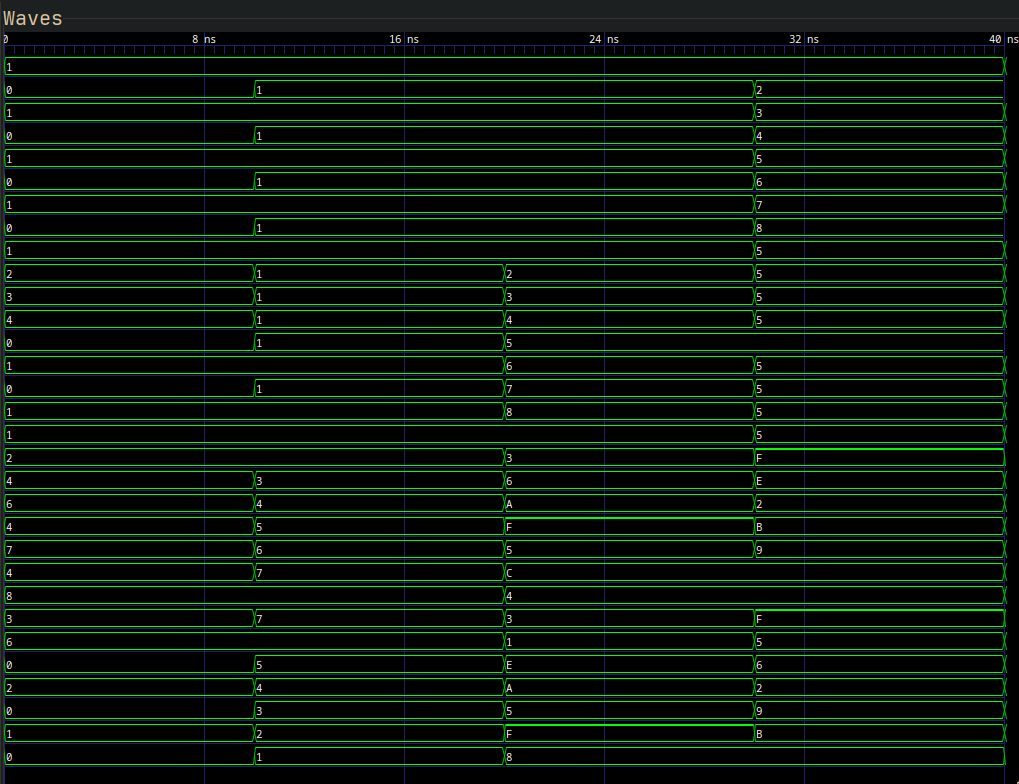
\includegraphics[width=1\linewidth]{figs/waveform_1.png}
    \label{fig:enter-label}
\end{figure}
\section{8-bit Full Adder}
\begin{itemize}
    \item \textbf{Inputs:}
    \begin{itemize}
        \item \texttt{[7:0] a} – First 8-bit number
        \item \texttt{[7:0] b} – Second 8-bit number 
        \item \texttt{carry$\_$in} – Input carry (1-bit)
    \end{itemize}
    \item \textbf{Outputs:}
    \begin{itemize}
        \item \texttt{[7:0] Sum} – 8-bit sum 
        \item \texttt{carry$\_$out} – Output carry (1-bit)
    \end{itemize}
\end{itemize}

\subsection*{Approach:}
An 8-bit full adder is constructed using eight 1-bit full adders in a ripple-carry configuration. FUll adder is implemented at each bit. A for-loop is used to implement this ripple-carry behavior behaviorally inside an \texttt{always} block. For each bit, the sum and carry are calculated as,

\begin{align*}
\texttt{sum[i]} &= A[i] \oplus B[i] \oplus \texttt{carry\_in}\\
\texttt{carry\_out} &= (A[i] \land B[i]) \lor (A[i] \land \texttt{carry\_in}) \lor (B[i] \land \texttt{carry\_in})
\end{align*}

The final carry becomes \texttt{carry$\_$out}.
\begin{figure}[!ht]
\centering
\resizebox{1\textwidth}{!}{%
\begin{circuitikz}
\tikzstyle{every node}=[font=\Large]
\draw (10.75,13) to[short] (12,13);
\draw (10.25,12) to[short] (12,12);
\draw  (12,13.25) rectangle (14,11.75);
\draw (14,12.5) to[short] (14.75,12.5);
\node [font=\Large] at (13,12.5) {XOR};
\draw (14.75,11.25) to[short] (16,11.25);
\draw (14.75,10.25) to[short] (16,10.25);
\draw  (16,11.5) rectangle (18,10);
\draw (18,10.75) to[short] (18.75,10.75);
\node [font=\Large] at (17,10.75) {XOR};
\draw (14.75,12.5) to[short] (14.75,11.25);
\draw (14.75,10.25) to[short] (10.75,10.25);
\draw (10.5,9) to[short] (12,9);
\draw (10.75,8) to[short] (12,8);
\draw  (12,9.25) rectangle (14,7.75);
\draw (14,8.5) to[short] (15.25,8.5);
\node [font=\Large] at (13,8.5) {AND};
\draw (10.75,13) to[short] (9.75,13);
\draw (9.5,8) to[short] (11,8);
\draw (9.75,13) to[short] (8.75,13);
\draw (10.25,12) to[short] (8.75,12);
\draw (10.75,10.25) to[short] (8.75,10.25);
\draw (9.5,11) to[crossing] (9.5,9.5);
\draw (9.5,9.5) to[short] (9.5,8);
\draw (10.5,13) to[crossing] (10.5,11);
\draw (10.5,11) to[crossing] (10.5,9.5);
\draw (10.5,9.5) to[short] (10.5,9);
\node [font=\Large] at (8.25,13) {A};
\node [font=\Large] at (8.25,12) {B};
\node [font=\Large] at (8.25,10.25) {$C_{in}$};
\draw (9,10.25) to[short] (9,5.75);
\draw (10.75,6.75) to[short] (12,6.75);
\draw (9,5.75) to[short] (12,5.75);
\draw  (12,7) rectangle (14,5.5);
\draw (14,6.25) to[short] (15.25,6.25);
\node [font=\Large] at (13,6.25) {AND};
\draw (10.75,6.75) to[short] (10.75,8);
\draw (9.5,11) to[short] (9.5,12);
\draw (10.5,9) to[crossing] (10.5,7);
\draw (10.5,7) to[crossing] (10.5,4.5);
\draw (10.5,4.5) to[short] (12,4.5);
\draw (10,3.5) to[short] (12,3.5);
\draw  (12,4.75) rectangle (14,3.25);
\draw (14,4) to[short] (19.25,4);
\node [font=\Large] at (13,4) {AND};
\draw (10,5.75) to[short] (10,3.5);
\draw (15.25,8) to[short] (16.5,8);
\draw (15.25,7) to[short] (16.5,7);
\draw  (16.5,8.25) rectangle (18.5,6.75);
\draw (18.5,7.5) to[short] (19.25,7.5);
\node [font=\Large] at (17.5,7.5) {OR};
\draw (19.25,6) to[short] (20.5,6);
\draw (19.25,5) to[short] (20.5,5);
\draw  (20.5,6.25) rectangle (22.5,4.75);
\draw (22.5,5.5) to[short] (23.25,5.5);
\node [font=\Large] at (21.5,5.5) {OR};
\draw (19.25,5) to[short] (19.25,4);
\draw (15.25,7) to[short] (15.25,6.25);
\draw (15.25,8) to[short] (15.25,8.5);
\draw (19.25,7.5) to[short] (19.25,6);
\node [font=\Large] at (19.5,10.75) {$SUM$};
\node [font=\Large] at (24,5.5) {$C_{out}$};
\end{circuitikz}
}%

\label{fig:my_label}
\end{figure}
\subsection*{code}
\begin{lstlisting}[style=style]
module bitadder(
  input [7:0] a,
  input [7:0] b,
  input carry_in,
  output reg [7:0] sum,
  output reg carry_out
);
reg carry;
integer i;

always @(*) begin
  carry = carry_in;
  for (i = 0; i < 8; i = i + 1) begin
    sum[i] = a[i] ^ b[i] ^ carry;
    carry = (a[i] & b[i]) | (a[i] & carry) | (b[i] & carry);
  end
  carry_out = carry;
end
endmodule
\end{lstlisting}
\subsection*{Testbench}

\begin{lstlisting}[style=style]
module tb_adder;
reg[7:0] a, b;
reg carry_in;
wire [7:0] sum;
wire carry_out;

bitadder uut(
  .a(a),
  .b(b),
  .carry_in(carry_in),
  .sum(sum),
  .carry_out(carry_out)
);
initial begin
  $dumpfile("8bitadder.vcd");
  $dumpvars(0, tb_adder);

  $display("Test Cases");
  // Test Case 1
  a = 8'b01101101; b = 8'b10110010; carry_in = 0;
  $monitor("%0t. %b  %b (%b)  %b (%b)",  $time, a, b, carry_in, sum, carry_out);
  #10

  // Test Case 2
  a = 8'b11010110; b = 8'b01010101; carry_in = 0;
  #10

  // Test Case 3
  a = 8'b11111111; b = 8'b00000001; carry_in = 0;
  #10

  // Test Case 4
  a = 8'b10011001; b = 8'b01101100; carry_in = 1;
  #10

  // Test Case 5
  a = 8'b01010101; b = 8'b11101010; carry_in = 1;
  #10

end
endmodule
\end{lstlisting}
Output of test bench,
\begin{lstlisting}[style = style]
Test Cases
0. 01101101  10110010 (0)  00011111 (1)
10. 11010110  01010101 (0)  00101011 (1)
20. 11111111  00000001 (0)  00000000 (1)
30. 10011001  01101100 (1)  00000110 (1)
40. 01010101  11101010 (1)  01000000 (1)
\end{lstlisting}
\pagebreak
\subsection*{Waveforms}
\begin{figure}[h!]
    \centering
    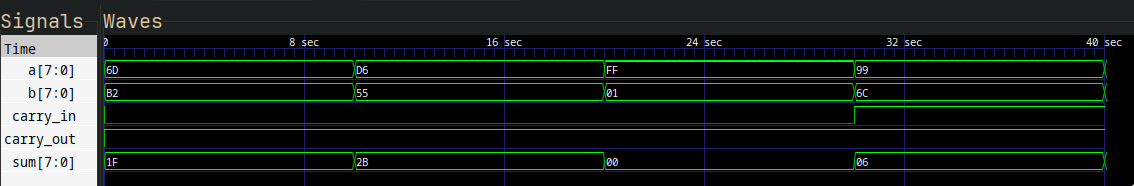
\includegraphics[width=1\linewidth]{figs/waveform_2.png}
    \label{fig:enter-label}
\end{figure}
\section{4-bit Adder using NAND Gates}
\begin{itemize}
    \item \textbf{Inputs:}
    \begin{itemize}
        \item \texttt{[3:0] A} – First 4-bit operand
        \item \texttt{[3:0] B} – Second 4-bit operand
        \item \texttt{carry$\_$in} – Initial carry-in (1-bit)
    \end{itemize}
    \item \textbf{Outputs:}
    \begin{itemize}
        \item \texttt{[3:0] Sum} – 4-bit sum of inputs
        \item \texttt{carry$\_$out} – Final carry-out (1-bit)
    \end{itemize}
\end{itemize}
\subsection*{Approach:}
A 4-bit ripple carry adder is constructed by chaining four 1-bit full adders. Each full adder is implemented using only 2-input NAND gates. The logic gates for XOR, AND, and OR are derived using NAND-only constructs. The same expressions for bitwise sum and carry are used as in the previous question, except instead of using XOR and OR gates directly, we have derived them using only fundamental NAND gates.
\subsection*{Logical Gates using NAND}
\subsubsection*{AND gate using NAND}
\begin{figure}[!h]
\centering
\resizebox{0.6\textwidth}{!}{%
\begin{circuitikz}
\tikzstyle{every node}=[font=\large]

\draw (8.75,15) to[short] (9,15);
\draw (8.75,14.5) to[short] (9,14.5);
\draw (9,15) node[ieeestd nand port, anchor=in 1, scale=0.89](port){} (port.out) to[short] (10.75,14.75);
\node [font=\large] at (8.5,15) {A};
\node [font=\large] at (8.5,14.5) {B};
\draw (12.5,15) to[short] (12.75,15);
\draw (12.5,14.5) to[short] (12.75,14.5);
\draw (12.75,15) node[ieeestd nand port, anchor=in 1, scale=0.89](port){} (port.out) to[short] (14.5,14.75);
\draw (11,15) to[short] (11,14.5);
\draw (11,14.5) to[short] (12.5,14.5);
\draw (11,15) to[short] (12.5,15);
\draw (14.5,14.75) to[short] (15,14.75);
\node [font=\large] at (15.5,14.75) {AB};
\end{circuitikz}
}%

\label{fig:my_label}
\end{figure}
Output of first NAND Gate is $\overline{A\cdot B}$. And passing it through both terminals of a two input NAND gate (which basically acts like a NOT gate) returns $A\cdot B$
\subsubsection*{OR gate using NAND}
\begin{figure}[!h]
\centering
\resizebox{0.6\textwidth}{!}{%
\begin{circuitikz}
\tikzstyle{every node}=[font=\large]
\draw (6.25,16.25) to[short] (6.5,16.25);
\draw (6.25,15.75) to[short] (6.5,15.75);
\draw (6.5,16.25) node[ieeestd nand port, anchor=in 1, scale=0.89](port){} (port.out) to[short] (8.25,16);
\draw (6.25,13.75) to[short] (6.5,13.75);
\draw (6.25,13.25) to[short] (6.5,13.25);
\draw (6.5,13.75) node[ieeestd nand port, anchor=in 1, scale=0.89](port){} (port.out) to[short] (8.25,13.5);
\draw (6.25,16.25) to[short] (6.25,15.75);
\draw (6.25,13.75) to[short] (6.25,13.25);
\draw (6.25,13.5) to[short] (5.75,13.5);
\draw (6.25,16) to[short] (5.75,16);
\draw (8.25,16) to[short] (8.75,16);
\draw (8.75,16) to[short] (8.75,15);
\draw (8.25,13.5) to[short] (8.75,13.5);
\draw (8.75,13.5) to[short] (8.75,14.5);
\draw (8.75,15) to[short] (10,15);
\draw (8.75,14.5) to[short] (10,14.5);
\draw (10,15) to[short] (10.25,15);
\draw (10,14.5) to[short] (10.25,14.5);
\draw (10.25,15) node[ieeestd nand port, anchor=in 1, scale=0.89](port){} (port.out) to[short] (12,14.75);
\node [font=\large] at (5.25,16) {A};
\node [font=\large] at (5.5,13.5) {B};
\node [font=\large] at (8.25,16.5) {$\overline{A}$};
\node [font=\large] at (8.25,13) {$\overline{B}$};
\node [font=\large] at (12.75,14.75) {$(\overline{\overline{A}\cdot\overline{B} }) $ };
\end{circuitikz}
}%

\label{fig:my_label}
\end{figure}
Inputs $A, B$ are duplicated and each (seperately) passed to a NAND gate, where they are inverted. The resultants are passed to another NAND gate where the final result is, $(\overline{\overline{A} \cdot \overline{B}})$ which simplifies (using De-Morgans Laws) to be, $A+B$

\subsubsection*{XOR using NAND}
\begin{figure}[h!]
\centering
\resizebox{1\textwidth}{!}{%
\begin{circuitikz}
\tikzstyle{every node}=[font=\large]
\draw (6.25,13.25) to[short] (6.5,13.25);
\draw (6.25,12.75) to[short] (6.5,12.75);
\draw (6.5,13.25) node[ieeestd nand port, anchor=in 1, scale=0.89](port){} (port.out) to[short] (8.25,13);
\draw (6.25,13.25) to[short] (6.25,14.5);
\draw (6.25,12.75) to[short] (6.25,11.25);
\draw (6.25,11.25) to[short] (5,11.25);
\draw (6.25,14.5) to[short] (5,14.5);
\draw (10,14.5) to[short] (10.25,14.5);
\draw (10,14) to[short] (10.25,14);
\draw (10.25,14.5) node[ieeestd nand port, anchor=in 1, scale=0.89](port){} (port.out) to[short] (12,14.25);
\draw (10,11.75) to[short] (10.25,11.75);
\draw (10,11.25) to[short] (10.25,11.25);
\draw (10.25,11.75) node[ieeestd nand port, anchor=in 1, scale=0.89](port){} (port.out) to[short] (12,11.5);
\draw (6.25,11.25) to[short] (10,11.25);
\draw (6.25,14.5) to[short] (10,14.5);
\draw (10,14) to[short] (10,11.75);
\draw (8.25,13) to[short] (10,13);
\draw (12,14.25) to[short] (13,14.25);
\draw (13,14.25) to[short] (13,13.25);
\draw (13,13.25) to[short] (13.75,13.25);
\draw (12,11.5) to[short] (13,11.5);
\draw (13,11.5) to[short] (13,12.75);
\draw (13,12.75) to[short] (13.75,12.75);
\draw (13.75,13.25) to[short] (14,13.25);
\draw (13.75,12.75) to[short] (14,12.75);
\draw (14,13.25) node[ieeestd nand port, anchor=in 1, scale=0.89](port){} (port.out) to[short] (15.75,13);
\node [font=\large] at (16.5,13) {$A \oplus B$};
\node [font=\large] at (4.5,14.5) {A};
\node [font=\large] at (4.5,11.25) {B};
\node [font=\large] at (8.5,13.25) {$\overline{AB}$};
\node [font=\large] at (12.5,14.75) {$\overline{A(\overline{AB})}$};
\node [font=\large] at (12.5,10.75) {$\overline{B(\overline{AB})}$};
\end{circuitikz}
}%

\label{fig:my_label}
\end{figure}

\subsubsection*{Worst Case Delay}
\begin{figure}
    \centering
    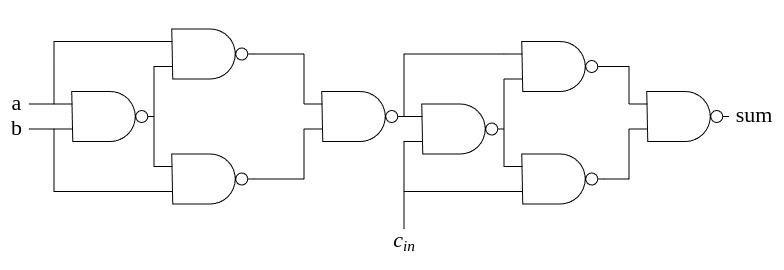
\includegraphics[width=1\linewidth]{figs/image.png}
    \caption{Sum}
    \label{fig:enter-label}
\end{figure}
\begin{figure}[!ht]
\centering
\resizebox{1\textwidth}{!}{%
\begin{circuitikz}
\tikzstyle{every node}=[font=\normalsize]



\draw (3,11) to[short] (3.25,11);
\draw (3,10.5) to[short] (3.25,10.5);
\draw (3.25,11) node[ieeestd nand port, anchor=in 1, scale=0.89](port){} (port.out) to[short] (5.25,10.75);
\draw (5.75,11) to[short] (6,11);
\draw (5.75,10.5) to[short] (6,10.5);
\draw (6,11) node[ieeestd nand port, anchor=in 1, scale=0.89](port){} (port.out) to[short] (7.75,10.75);
\draw (8.25,11) to[short] (8.5,11);
\draw (8.25,10.5) to[short] (8.5,10.5);
\draw (8.5,11) node[ieeestd nand port, anchor=in 1, scale=0.89](port){} (port.out) to[short] (10.25,10.75);
\draw (5.25,10.75) to[short] (5.75,10.75);
\draw (5.75,11) to[short] (5.75,10.5);
\draw (8.25,11) to[short] (8.25,10.5);


\draw (3,9.5) to[short] (3.25,9.5);
\draw (3,9) to[short] (3.25,9);
\draw (3.25,9.5) node[ieeestd nand port, anchor=in 1, scale=0.89](port){} (port.out) to[short] (5.25,9.25);
\draw (5.75,9.5) to[short] (6,9.5);
\draw (5.75,9) to[short] (6,9);
\draw (6,9.5) node[ieeestd nand port, anchor=in 1, scale=0.89](port){} (port.out) to[short] (7.75,9.25);
\draw (8.25,9.5) to[short] (8.5,9.5);
\draw (8.25,9) to[short] (8.5,9);
\draw (8.5,9.5) node[ieeestd nand port, anchor=in 1, scale=0.89](port){} (port.out) to[short] (10.25,9.25);
\draw (5.25,9.25) to[short] (5.75,9.25);
\draw (5.75,9.5) to[short] (5.75,9);
\draw (8.25,9.5) to[short] (8.25,9);


\draw (3,7.75) to[short] (3.25,7.75);
\draw (3,7.25) to[short] (3.25,7.25);
\draw (3.25,7.75) node[ieeestd nand port, anchor=in 1, scale=0.89](port){} (port.out) to[short] (5.25,7.5);
\draw (5.75,7.75) to[short] (6,7.75);
\draw (5.75,7.25) to[short] (6,7.25);
\draw (6,7.75) node[ieeestd nand port, anchor=in 1, scale=0.89](port){} (port.out) to[short] (7.75,7.5);
\draw (8.25,7.75) to[short] (8.5,7.75);
\draw (8.25,7.25) to[short] (8.5,7.25);
\draw (8.5,7.75) node[ieeestd nand port, anchor=in 1, scale=0.89](port){} (port.out) to[short] (10.25,7.5);
\draw (5.25,7.5) to[short] (5.75,7.5);
\draw (5.75,7.75) to[short] (5.75,7.25);
\draw (8.25,7.75) to[short] (8.25,7.25);
\draw (10.25,10.75) to[short] (10.75,10.75);
\draw (10.25,9.25) to[short] (10.75,9.25);
\draw (10.75,10.75) to[short] (10.75,10.25);
\draw (10.75,9.75) to[short] (10.75,9.25);
\draw (10.25,7.5) to[short] (13,7.5);
\draw (10.75,10.25) to[short] (11,10.25);
\draw (10.75,9.75) to[short] (11,9.75);
\draw (11,10.25) node[ieeestd nand port, anchor=in 1, scale=0.89](port){} (port.out) to[short] (12.75,10);
\draw (7.75,10.75) to[short] (8.25,10.75);
\draw (7.75,9.25) to[short] (8.25,9.25);
\draw (7.75,7.5) to[short] (8.25,7.5);
\draw (13.25,10.25) to[short] (13.25,9.75);
\draw (13.5,10.25) to[short] (13.75,10.25);
\draw (13.5,9.75) to[short] (13.75,9.75);
\draw (13.75,10.25) node[ieeestd nand port, anchor=in 1, scale=0.89](port){} (port.out) to[short] (15.5,10);
\draw (13,7.75) to[short] (13,7.25);
\draw (13.5,7.75) to[short] (13.75,7.75);
\draw (13.5,7.25) to[short] (13.75,7.25);
\draw (13.75,7.75) node[ieeestd nand port, anchor=in 1, scale=0.89](port){} (port.out) to[short] (15.5,7.5);
\draw (16,8) to[short] (16.25,8);
\draw (16,7.5) to[short] (16.25,7.5);
\draw (16.25,8) node[ieeestd nand port, anchor=in 1, scale=0.89](port){} (port.out) to[short] (18,7.75);
\draw (16,10) to[short] (16,8);
\node [font=\normalsize] at (2.75,11) {A};
\node [font=\normalsize] at (2.75,10.5) {B};
\node [font=\normalsize] at (2.75,9.5) {A};
\node [font=\normalsize] at (2.75,9) {$C_{in}$};
\node [font=\normalsize] at (2.75,7.75) {B};
\node [font=\normalsize] at (2.75,7.25) {$C_{in}$};
\node [font=\normalsize] at (18.85,7.75) {$C_{out}$};
\draw (13,7.75) to[short] (13.5,7.75);
\draw (13,7.25) to[short] (13.5,7.25);
\draw (15.5,10) to[short] (16,10);
\draw (15.5,7.5) to[short] (16.25,7.5);
\draw (13.25,10.25) to[short] (13.75,10.25);
\draw (13.25,9.75) to[short] (13.75,9.75);
\draw (12.75,10) to[short] (13.25,10);
\end{circuitikz}
}%
\caption{Carry}
\label{fig:my_label}
\end{figure}
There are 6 levels of combinational logics that occur sequentially for calculation of each bit of "sum", there will be the same number of levels in case of "carry$\_$out". The maximum delay will occur regardless of $a, b$ as long as one of them are $HIGH$, and $c_{in}$ toggles. This causes a propagation delay in each and every level of the circuit, and since we have taken delay as $1ns$ at each gate, total delay will be equal to number of levels, as delay propagates parallelly through all the gates in each level. So here, total delay will be $6ns$. This is for a singular bit, since we are dealing with 4-bit numbers, total delay comes out to be $24ns$ which is what we observe through the timing diagram.
We have taken the consecutive test cases, $a=0, b = 0, c_{in} = 0$ and $a = 15, b = 0, c_{in} = 1$. here, $c_{in}$ toggles for every bit from the former to the later test case, so observe the waveform for maximum delay. \newline 
In case of "sum", there are 6 levels again, between the two test cases since the delay for each bit is $6ns$ which is also the maximum possible delay which can occur for "sum" bit, the sum calculated within $6ns$ itself. Since a 4-bit sum requires only 3 carrys to be calculated, before it can be computed, it requires $18ns$ to compute. As for the last bit, it only requires $3ns$ as $a \oplus b$ would have already been calculated. So a total delay of $21ns$ is observed for the sum.
\subsection*{Code}
\begin{lstlisting}[style=style]
`timescale 1ns/1ns

module and_nand(
  input a,
  input b,
  output out
);
wire temp;
nand #1(temp, a, b);
nand #1(out, temp, temp);
endmodule

module or_nand(
  input a,
  input b,
  output out
);
wire temp1, temp2;
nand #1(temp1, a, a);
nand #1(temp2, b, b);
nand #1(out, temp1, temp2);
endmodule

module xor_nand(
  input a,
  input b,
  output out
);
wire temp1, temp2, temp3;
nand #1(temp1, a, b);
nand #1(temp2, a, temp1);
nand #1(temp3, b, temp1);
nand #1(out, temp2, temp3);
endmodule

module bitadder(
  input [3:0] a,
  input [3:0] b,
  input carry_in,
  output [3:0] sum,
  output carry_out
);
wire [4:0] carry;    
assign carry[0] = carry_in;


genvar i;
generate
  for (i = 0; i < 4; i = i + 1) begin
    wire temp1, temp2, temp3, temp4, temp5;

    xor_nand xor1 (.a(a[i]), .b(b[i]), .out(temp1));
    xor_nand xor2 (.a(temp1), .b(carry[i]), .out(sum[i]));

    and_nand and1 (.a(a[i]), .b(b[i]), .out(temp2));
    and_nand and2 (.a(a[i]), .b(carry[i]), .out(temp3));
    and_nand and3 (.a(b[i]), .b(carry[i]), .out(temp4));

    or_nand or1 (.a(temp2), .b(temp3), .out(temp5));
    or_nand or2 (.a(temp5), .b(temp4), .out(carry[i+1]));
  end
endgenerate

assign carry_out = carry[4];

endmodule
\end{lstlisting}
\subsection*{Testbench}
\begin{lstlisting}[style=style]
module tb_adder;
reg [3:0] a, b;
reg carry_in;
wire [3:0] sum;
wire carry_out;

bitadder uut (
  .a(a),
  .b(b),
  .carry_in(carry_in),
  .sum(sum),
  .carry_out(carry_out)
);
initial begin
  $dumpfile("4bitadder.vcd");
  $dumpvars(0, tb_adder);
  
  // Test Case 1
  a = 4'b0000; b = 4'b0000; carry_in = 0;
  #50
  

  // Test Case 2 
  $display("%0t %b  %b (%b)  %b (%b)", $time, a, b, carry_in, sum, carry_out);
  $display("done");

  a = 4'b1111; b = 4'b0000; carry_in = 1;
  #50

  // Test Case 3
  $display("%0t %b  %b (%b)  %b (%b)", $time, a, b, carry_in, sum, carry_out);
  $display("done");

  a = 4'b1111; b = 4'b1111; carry_in = 0;
  #50

  // Test Case 4
  $display("%0t %b  %b (%b)  %b (%b)", $time, a, b, carry_in, sum, carry_out);
  $display("done");

  a = 4'b0000; b = 4'b0000; carry_in = 1;
  #50

  // Test Case 5 
  $display("%0t %b  %b (%b)  %b (%b)", $time, a, b, carry_in, sum, carry_out);
  $display("done");

  a = 4'b1010; b = 4'b0101; carry_in = 0;
  #50 
  $display("%0t %b  %b (%b)  %b (%b)", $time, a, b, carry_in, sum, carry_out);

end
endmodule
\end{lstlisting}
Output of test bench,
\begin{lstlisting}[style = style]
    50 0000  0000 (0)  0000 (0)
done
100 1111  0000 (1)  0000 (1)
done
150 1111  1111 (0)  1110 (1)
done
200 0000  0000 (1)  0001 (0)
done
250 1010  0101 (0)  1111 (0)
\end{lstlisting}
\subsection*{Waveforms}
\begin{figure}[h!]
    \centering
    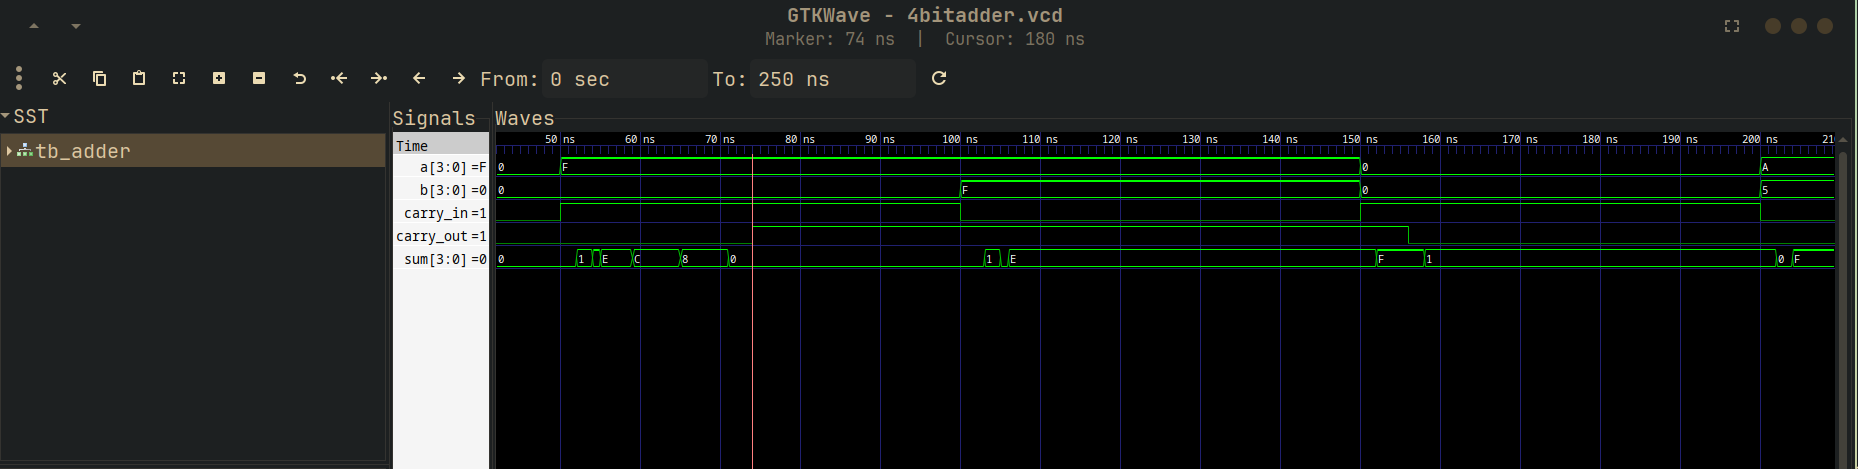
\includegraphics[width=1\linewidth]{figs/waveform_3.png}
    \label{fig:enter-label}
\end{figure}
\end{document}

